\begin{figure}[tbp]
  \centering
  {\small
    Linear part: $C_0\xrightarrow{d_1}C_1\xrightarrow{d_1}C_2$,
    \quad $H_a=H^a(C_\bullet,d_1)$.\par}
  \medskip
  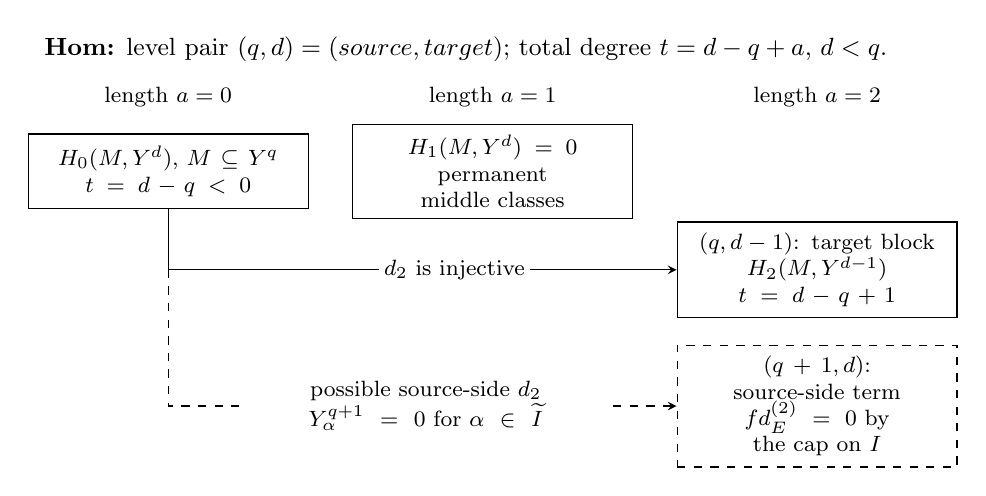
\begin{tikzpicture}[
      x=.01\linewidth,y=1cm,
      every node/.style={font=\footnotesize,align=center},
      term/.style={text width=.27\linewidth,inner sep=4pt},
      permanent/.style={term,draw,semithick,minimum height=.95cm},
      endpoint/.style={term,draw,thin,minimum height=.95cm},
      excluded/.style={term,draw,dashed,thin,minimum height=.95cm},
      differential/.style={->,thin,>=stealth}
    ]
    \node[anchor=west,align=left,font=\small] at (-14,-4.55)
      {\textbf{Hom:} level pair $(q,d)=(\text{source},\text{target})$;
        total degree $t=d-q+a$, $d<q$.};
    \node at (0,-5.16) {length $a=0$};
    \node at (34,-5.16) {length $a=1$};
    \node at (68,-5.16) {length $a=2$};
    \node[endpoint] (hom-zero) at (0,-6.1)
      {$H_0(M,Y^d)$, $M\subseteq Y^q$\\$t=d-q<0$};
    \node[permanent] (hom-middle) at (34,-6.1)
      {$H_1(M,Y^d)=0$\\permanent middle classes};
    \node[endpoint] (hom-target) at (68,-7.35)
      {$(q,d-1)$: target block\\$H_2(M,Y^{d-1})$\\$t=d-q+1$};
    \node[excluded] (hom-source) at (68,-9.08)
      {$(q+1,d)$: source-side term\\$f d_E^{(2)}=0$ by the cap on $I$};
    \draw[differential] (hom-zero.south) -- (0,-7.35)
      -- (hom-target.west);
    \node[fill=white,inner sep=2pt] at (30,-7.35)
      {$d_2$ is injective};
    \draw[differential,dashed] (0,-7.35) -- (0,-9.08)
      -- (hom-source.west);
    \node[fill=white,text width=.38\linewidth,inner sep=2pt] at (27,-9.08)
      {possible source-side $d_2$\\
        $Y^{q+1}_\alpha=0$ for $\alpha\in\widetilde I$};
  \end{tikzpicture}
  \caption{The Hom length filtration for a direct summand $M$ of $Y^q$
    supported on $\widetilde I$, with the family capped at $q$ on $I$.
    Here $d<q$, and $H_a$ denotes the linear cohomology $\mathsf H_a$ with
    family and bidegree indices suppressed.  The secondary differential
    of a length-zero linear cocycle $f$ has the two displayed target blocks;
    $d_E^{(2)}$ denotes the length-two part of the source differential.
    The source-side contribution
    $f d_E^{(2)}$ vanishes: length-two paths are diagonal and the cap
    excludes level-$q+1$ source generators on $\widetilde I$.
    Higher source generators outside $I$ need not vanish.
    Negative-degree actual Hom vanishes, forcing injection into the
    remaining target block.  The identity and token classes give the
    middle vanishing proved in Lemma~\ref{lem:rigidity-hom-filtration}.
    The dashed arrow marks an excluded possibility.}
  \label{fig:hom-filtration}
\end{figure}
